\documentclass[../tech_report_1.tex]{subfiles}
\graphicspath{{img/}{../img/}}
\begin{document}

\section{Spherical k-means clustering}

Spherical k-means clustering is the same idea, however, the points are not on a flat euclidean space but rather on the hypersphere.
We investigated a MATLAB implementation by Nguyen  \cite{nguyen2008gene,nguyen_spherical_clustering},
which required a mean-and-norm-normalized dataset located on a hypersphere.
Important aspects of this implementation include:
\begin{itemize}
\item When there exists an empty cluster, the largest cluster is split
\item Use the dot product as ``negative distance'', which leverages the
fact that observations are unit vectors on the hypersphere
\item Use the normalized sum of observations as a centroid/mean, which leverages
the fact that observations are unit vectors on the hypersphere. Note
that this fails on pathological cases where the sum of observations
is zero.
For example, if you have two vectors that are opposite of each other, their sum is the zero vector.
\end{itemize}

\subsection{Our investigation}

In order to test how well the spherical k-means clustering algorithm
worked, we constructed a random data set using the Von Mises distribution
random sampling function from the MATLAB Circular Statistics Toolbox  \cite{circstats}.
We constructed 70 clusters of 10 points each, using random points
on the sphere as means and with step size $\kappa=100$, and then applied the spherical k-means clustering and visualized the results on the unit
three dimensional sphere, color coded for each cluster and with estimated
means labeled as red $X$'s and true means labeled as black $X$'s.


% TODO: fix graphics (reduce numer of clusters, put legend on the plot, figure caption, background off)

\begin{figure}[ht]
\caption{Plot of 10 clusters and means on a 3-D sphere}
\caption{Plot of 10 clusters and means on a 3-D sphere. Red x's are computed means, black x's are actual means; because they line up fairly well, the implementation is effective.}
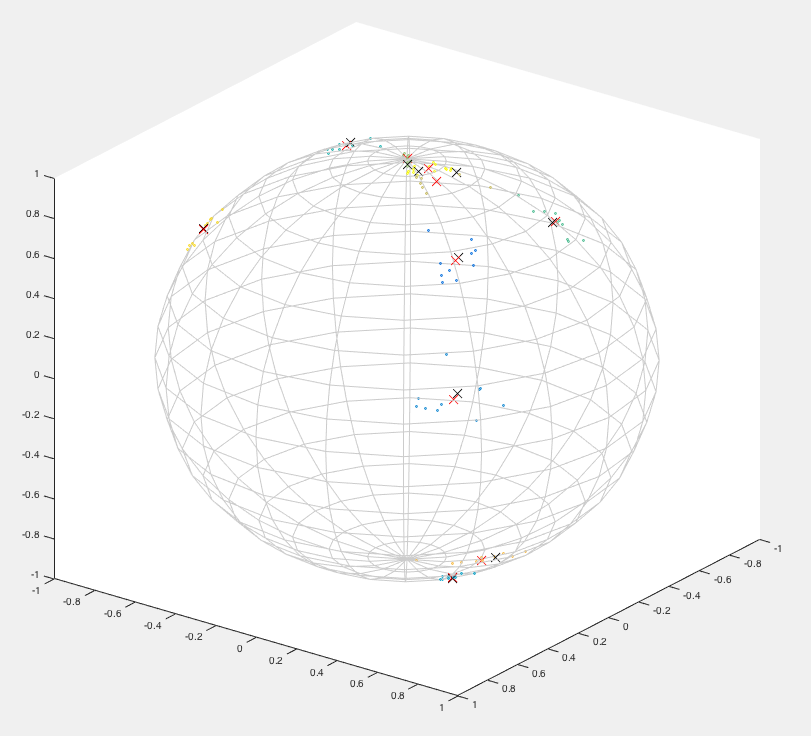
\includegraphics[width=1\textwidth]{sphere_points_10_clusters}
\end{figure}

\begin{figure}[ht]
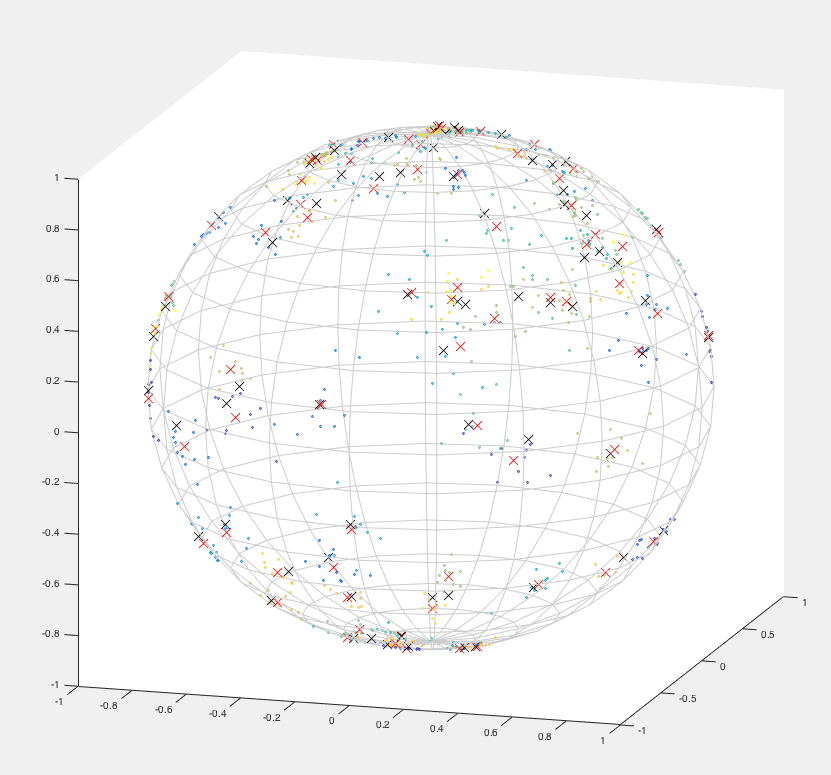
\includegraphics[width=1\textwidth]{sphere_points_70_clusters}
\caption{Same experiment with 70 clusters number of clusters.}
\end{figure}


\end{document}
